\documentclass[12pt,t]{beamer}
\usepackage{graphicx}
\usepackage[vlined]{algorithm2e}
\usepackage{times}
\usepackage{bbold}
\usepackage{calc}
\usepackage{url}
\usepackage{soul}
\usepackage{graphicx}
\usepackage{multirow, hhline}
\usepackage{array, booktabs}
\usepackage{amsmath}
\usepackage{amssymb}
\usepackage{relsize}
\usepackage{multirow}
\usepackage{booktabs}
\usepackage{pagecolor}
\usepackage{lipsum}
\usepackage{capt-of}
\usepackage{booktabs}

\usepackage{graphicx}
\usepackage{multicol}
\usepackage[T1]{fontenc}
\usepackage{ae}
\graphicspath{{fig/}}
\setbeameroption{hide notes}
\setbeamertemplate{note page}[plain]

\usetheme{default}
\beamertemplatenavigationsymbolsempty
\hypersetup{pdfpagemode=UseNone}

\usefonttheme{professionalfonts}
\usefonttheme{serif}
\usepackage{fontspec}
\setmainfont{Karla}
\setbeamerfont{note page}{family*=pplx,size=\footnotesize} % Palatino for notes

\definecolor{foreground}{RGB}{70,70,70}
\definecolor{background}{RGB}{249, 249, 249} %24,24,24
%\definecolor{title}{RGB}{107,174,214} %107,174,214
\definecolor{title}{RGB}{70,70,70}
\definecolor{gray}{RGB}{0,0,0}
\definecolor{subtitle}{RGB}{70,70,70}
\definecolor{hilight}{RGB}{102,255,204}
\definecolor{vhilight}{RGB}{255,111,207}

\setbeamercolor{titlelike}{fg=title}
\setbeamercolor{subtitle}{fg=subtitle}
\setbeamercolor{institute}{fg=gray}
\setbeamercolor{normal text}{fg=foreground,bg=background}


\setbeamercolor{item}{fg=foreground} % color of bullets
\setbeamercolor{subitem}{fg=gray}
\setbeamercolor{itemize/enumerate subbody}{fg=gray}
\setbeamertemplate{itemize subitem}{{\textendash}}
\setbeamerfont{itemize/enumerate subbody}{size=\footnotesize}
\setbeamerfont{itemize/enumerate subitem}{size=\footnotesize}

\setbeamercolor{block title}{fg=white,bg=gray!70}
\setbeamercolor{block body}{fg=black,bg=gray!10}
\setbeamercolor{block title alerted}{fg=red,bg=gray!40}
\setbeamercolor{block title example}{fg=black,bg=green!20}
\setbeamercolor{block body example}{fg=black,bg=green!5}
\setbeamerfont{block title}{series=\bfseries}

\hypersetup{colorlinks,linkcolor=foreground,urlcolor=foreground}


\setbeamertemplate{footline}{%
    \raisebox{5pt}{\makebox[\paperwidth]{\hfill\makebox[20pt]{\color{gray}
          \scriptsize\insertframenumber}}}\hspace*{5pt}}

\addtobeamertemplate{note page}{\setlength{\parskip}{12pt}}


\newcommand{\bi}{\begin{itemize}}
\newcommand{\ei}{\end{itemize}}
\newcommand{\ig}{\includegraphics}
\newcommand{\subt}[1]{{\footnotesize \color{subtitle} {#1}}}

\let\emph\relax % there's no \RedeclareTextFontCommand
\DeclareTextFontCommand{\emph}{\bfseries\em}


\setbeamertemplate{frametitle}
{\vskip4pt
  \leavevmode
%\hbox{%
\begin{beamercolorbox}[wd=\paperwidth,ht=2ex,dp=0ex]{frametitle}%
\underline{\makebox[\paperwidth][l]{\hspace*{10pt}
\large {{\insertframetitle}}}}
\end{beamercolorbox}
%  }%
}

%\setbeamercolor{frametitle}{fg=yellow,bg=red}

\begin{document}

\AtBeginSection[]{
  \begin{frame}
  \vfill
  \centering
  \begin{beamercolorbox}[sep=8pt,center,shadow=true,rounded=true]{title}
    \underline{\makebox[0.6\paperwidth][l]{
\large {{\insertsectionhead}}}}
  \end{beamercolorbox}
  \vfill
  \end{frame}
}

\title{\large{Lecture \#16: Boosting}}
\subtitle{CS 109A, STAT 121A, AC 209A: Data Science}
\author{Pavlos Protopapas \and Kevin Rader}
%\institute{Harvard University}
\date{}
\titlegraphic{
   
\includegraphics[height=2cm]{iacs}
\includegraphics[height=2cm]{hogwarts}
}
{
\setbeamertemplate{footline}{} % no page number here
\frame{
  \titlepage
  
}
}


\begin{frame}{Lecture Outline}
\tableofcontents
\end{frame}

%%%%%%%%%%%%%%%%%%%%%%%%%%%%%%%%%%%%%%%%%%%%%%%%%%%%%%%%%%%%%%%%%%%%%%%%%%%%%%
\section{Review}

%%%%%%%%%%%%%%
\begin{frame}{Bags and Forests of Trees} 
\only<1>{
Last time we examined how the short-comings of single decision tree models can be overcome by ensemble methods - making one model out of many trees.
\vskip0.2cm
We focused on the problem of training large trees, these models have low bias but high variance. 
\vskip0.2cm
We compensated by training an ensemble of full decision trees and then averaging their predictions - thereby reducing the variance of our final model.
}

\only<2>{
\begin{itemize}
\item Bagging:
\begin{itemize}
\item create an ensemble of full trees, each trained on a bootstrap sample of the training set; 
\item average the predictions
\end{itemize}
\vskip0.2cm
\item Random forest:
\begin{itemize}
\item create an ensemble of full trees,each trained on a bootstrap sample of the training set; 
\item in each tree and each split, randomly select a subset of predictors, choose a predictor from this subset for splitting; 
\item average the predictions
\end{itemize}
\vskip0.2cm
Note that the ensemble building aspects of both method are embarrassingly parallel!
\end{itemize}
}

\end{frame}

\begin{frame}{Motivation for Boosting}
Could we address the shortcomings of single decision trees models in some other way? 
\vskip0.2cm
For example, rather than performing variance reduction on complex trees, can we decrease the bias of simple trees - make them more expressive? 
\vskip0.2cm
An solution to this problem, making an expressive model from simple trees, is another class of ensemble methods called \emph{boosting}.
\end{frame}


%%%%%%%%%%%%%%%%%%%%%%%%%%%%%%%%%%%%%%%%%%%%%%%%%%%%%%%%%%%%%%%%%%%%%%%%%%%%%%
\section{Boosting Algorithms}

\subsection{Gradient Boosting}
%%%%%%%%%%%%%%
\begin{frame}{Gradient Boosting} 
\only<1>{
The key intuition behind boosting is that one can take an ensemble of simple models $\{T_h\}_{h\in H}$ and additively combine them into a single, more complex model.
\vskip0.2cm
Each model $T_h$ might be a poor fit for the data, but a linear combination of the ensemble
\[
T = \sum_h \lambda_h T_h
\]
can be expressive.
\vskip0.2cm
But which models should we include in our ensemble? What should the coefficients or weights in the linear combinations be?
}

\only<2->{
\vskip-0.4cm
\scriptsize
\emph{Gradient boosting} is a method for iteratively building a complex regression model $T$ by adding simple models. Each new simple model added to the ensemble compensates for the weaknesses of the current ensemble.
\vskip0.2cm
\begin{enumerate}
\pause
\item Fit a simple model $T^{(0)}$ on the training data
\[
\{(x_1, y_1),\ldots, (x_N, y_N)\}.
\]
Set $T \leftarrow T^{(0)}$. 
\vskip0.2cm
Compute the residuals $\{r_1, \ldots, r_N\}$ for $T$. 
\vskip0.2cm
\pause
\item Fit a simple model, $T^{i}$, to the current \emph{residuals}, i.e. train using
\[
\{(x_1, r_1),\ldots, (x_N, r_N)\}.
\]
\vskip0.2cm
\pause
\item Set $T\leftarrow T + \lambda T^{i}$
\vskip0.2cm
\pause
\item Compute residuals, set $r_n\leftarrow r_n - \lambda T^{i}(x_n), \; n= 1,\ldots, N$
\item Repeat steps 2-4 until \emph{stopping} condition met
\end{enumerate}
\vskip0.2cm
where $\lambda$ is a constant called the \emph{learning rate}.
}
\end{frame}

%%%%%%%%%%%%%%
\begin{frame}{Why Does Gradient Boosting Work?} 
Intuitively, each simple model $T^{(i)}$ we add to our ensemble model $T$ models the errors of $T$. 
\vskip0.2cm
Thus, with each addition of $T^{(i)}$, the residual is reduced 
\[
r_n - \lambda T^{(i)}(x_n).
\]
\vskip0.2cm
Note that gradient boosting has a tuning parameter, $\lambda$. 
\vskip0.2cm
If we want to easily reason about how to choose $\lambda$ and investigate the effect of $\lambda$ on the model $T$, we need a bit more mathematical formalism.
\vskip0.2cm
In particular, we need to formulate gradient boosting as a type of \emph{gradient descent}.
\end{frame}

\subsection{Relation to Gradient Descent}
%%%%%%%%%%%%%%
\begin{frame}{A Brief Sketch of Gradient Descent} 
\only<1>{
In optimization, when we wish to minimize a function, called the \emph{objective function}, over a set of variables, we compute the partial derivatives of this function with respect to the variables. 
\vskip0.2cm
If the partial derivatives are sufficiently simple, one can analytically find a common root - i.e. a point at which all the partial derivatives vanish; this is called a \emph{stationary point}
\vskip0.2cm
If the objective function has the property of being \emph{convex}, then the stationary point is precisely the min.
}

\only<2>{
\vskip-0.4cm
\footnotesize
In practice, our objective functions are complicated and analytically find the stationary point is intractable.
\vskip0.2cm
Instead, we use an iterative method called \emph{gradient descent}:
\begin{enumerate}
\item initialize the variables at any value
\[
x = [x_0, \ldots, x_J]
\]
\item take the gradient of the objective function at the current variable values 
\[
\nabla f(x) = \left[\frac{\partial f}{\partial x_1}(x), \ldots, \frac{\partial f}{\partial x_J}(x)\right]
\]
\item adjust the variables values by some negative multiple of the gradient
\[
x \leftarrow x- \lambda \nabla f(x)
\]
\end{enumerate}
\vskip0.2cm
The factor $\lambda$ is often called the learning rate.
}

\end{frame}

%%%%%%%%%%%%%%
\begin{frame}{Why Does Gradient Descent Work?} 
\only<1>{
\small
\vskip-0.4cm
\textbf{Claim:} If the function is convex, this iterative methods will eventually move $x$ close enough to the minimum, for an appropriate choice of $\lambda$.
\vskip0.2cm
\textbf{Why does this work?} Recall, that as a vector, the gradient at at point gives the direction for the greatest possible rate of increase. 

\begin{center}
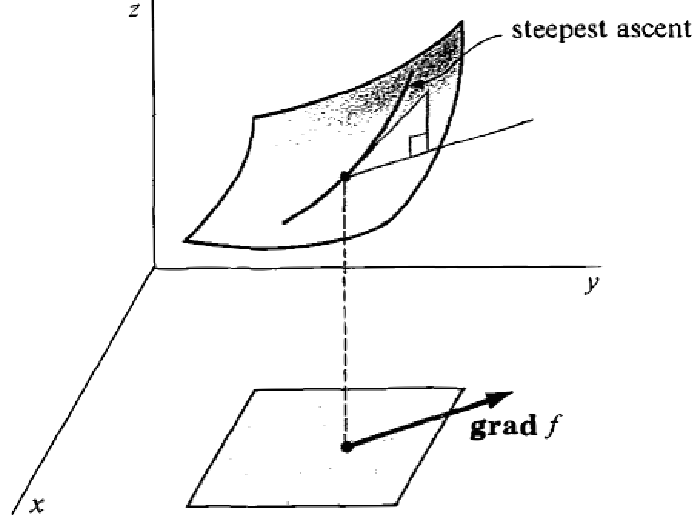
\includegraphics[width=60mm]{lecture16_g1}
\end{center}
}

\only<2>{
\vskip-0.4cm
Subtracting a $\lambda$ multiple of the gradient from $x$, moves $x$ in the \emph{opposite} direction of the gradient (hence towards the steepest decline) by a step of size $\lambda$.  
\vskip0.2cm
If $f$ is convex, and we keep taking steps descending on the graph of $f$, we will eventually reach the minimum.
\begin{center}
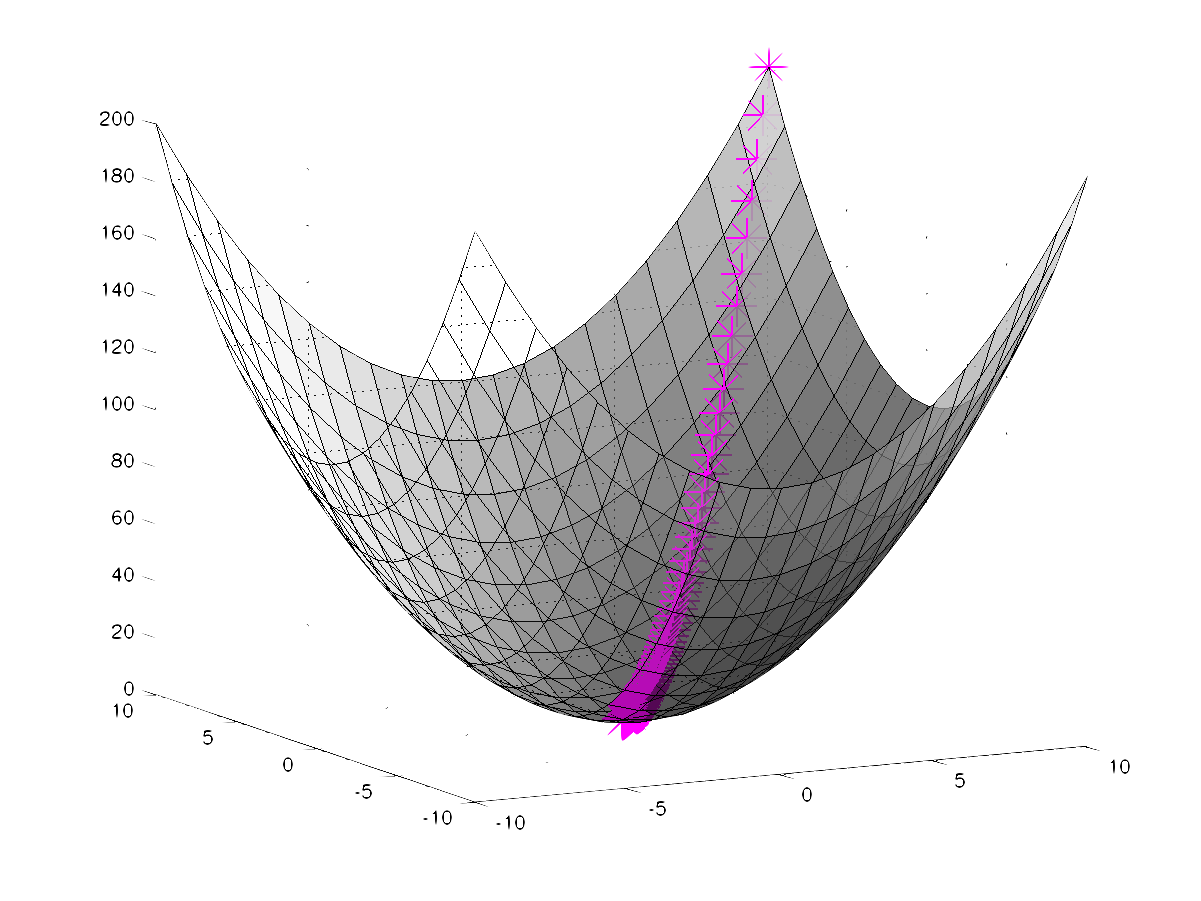
\includegraphics[width=60mm]{lecture16_g2}
\end{center}
}
\end{frame}

%%%%%%%%%%%%%%
\begin{frame}{Gradient Boosting as Gradient Descent} 
\only<1>{
\small
\vskip-0.4cm
Often in regression, our objective is to minimize the MSE
\[
\text{MSE}(\hat{y}_1, \ldots, \hat{y}_N) = \frac{1}{n} \sum_{i=n}^N(y_n - \hat{y}_n)^2
\]
Treating this as an optimization problem, we can try to directly minimize the MSE with respect to the predictions
\begin{align*}
\nabla \text{MSE} &= \left[ \frac{\partial \text{MSE}}{\partial \hat{y}_N}, \ldots, \frac{\partial \text{MSE}}{\partial \hat{y}_N}\right]\\
&= -2 \left[ y_1 - \hat{y}_1, \ldots, y_N - \hat{y}_N\right]\\
&= -2 \left[r_1, \ldots, r_N\right]
\end{align*}
The update step for gradient descent would look like
\[
\hat{y}_n \leftarrow \hat{y}_n + \lambda r_n,\quad n = 1, \ldots, N
\]
}
\only<2>{
There is two reasons why minimizing the MSE with respect to $\hat{y}_n$'s is not interesting:
\vskip0.2cm
\begin{itemize}
\item We know where the minimum MSE occurs: $\hat{y}_n = y_n$, for every $n$.
\vskip0.2cm
\item Learning sequences of predictions, $\hat{y}^{1}_n, \ldots, \hat{y}^{i}_n, \ldots$, does not produce a model. The predictions in the sequences do not depend on the predictors!
\end{itemize}
}
\only<3>{
\vskip-0.4cm
The solution is to change the update step in gradient descent. Instead of using the gradient - the residuals - we use an \emph{approximation} of the gradient that depends on the predictors:
\[
\hat{y} \leftarrow \hat{y}_n + \lambda \hat{r}_n(x_n),\quad n = 1, \ldots, N
\]
In gradient boosting, we use a simple model to approximate the residuals, $\hat{r}_n(x_n)$, in each iteration.
\vskip0.2cm
\textbf{Motto:} gradient boosting is a form of gradient descent with the MSE as the objective function. 
\vskip0.2cm
\textbf{Technical note:} note that gradient boosting is descending in a space of models or functions relating $x_n$ to $y_n$!
}

\only<4>{
But why do we care that gradient boosting is gradient descent?
\vskip0.2cm
By making this connection, we can import the massive amount of techniques for studying gradient descent to analyze gradient boosting.
\vskip0.2cm
For example, we can easily reason about how to choose the learning rate $\lambda$ in gradient boosting.
}
\end{frame}


%%%%%%%%%%%%%%
\begin{frame}{Choosing a Learning Rate} 
\only<1>{
\vskip-0.4cm
Under ideal conditions, gradient descent iteratively approximates and converges to the optimum. 
\vskip0.2cm
\emph{When do we terminate gradient descent?} 
\vskip0.2cm
\begin{itemize}
\item We can limit the number of iterations in the descent. But for an arbitrary choice of maximum iterations, we cannot guarantee that we are sufficiently close to the optimum in the end.
\vskip0.2cm
\item If the descent is stopped when the updates are sufficiently small (e.g. the residuals of $T$ are small), we encounter a new problem: the algorithm may never terminate!
\end{itemize}
\vskip0.2cm
Both problems have to do with the magnitude of the learning rate, $\lambda$.
}
\only<2>{
For a constant learning rate, $\lambda$, if $\lambda$ is too small, it takes too many iterations to reach the optimum.
\begin{center}
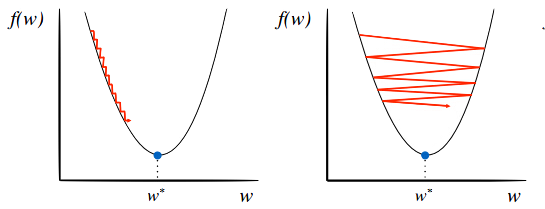
\includegraphics[width=100mm]{lecture16_g4}
\end{center}
If $\lambda$ is too large, the algorithm may `bounce' around the optimum and never get sufficiently close.
}

\only<3>{
Choosing $\lambda$:
\begin{itemize}
\item If $\lambda$ is a constant, then it should be tuned through cross validation.
\item For better results, use a variable $\lambda$. That is, let the value of $\lambda$ depend on the gradient
\[
\lambda = h(\| \nabla f(x)\|), 
\]
where $\|\nabla f(x)\|$ is the magnitude of $\nabla f(x)$. So
\vskip0.2cm
\begin{itemize}
\item around the optimum, when the gradient is small, $\lambda$ should be small
\item far from the optimum, when the gradient is large, $\lambda$ should be larger
\end{itemize}
\end{itemize}
}
\end{frame}

\subsection{AdaBoost}

%%%%%%%%%%%%%%
\begin{frame}{Motivation for AdaBoost} 
\only<1>{
\vskip-0.4cm
Using the language of gradient descent also allow us to connect gradient boosting for regression to a boosting algorithm often used for classification, AdaBoost.
\vskip0.2cm
In classification, we typically want to minimize the classification error:
\[
\text{Error} = \frac{1}{N} \sum_{n=1}^N \mathbb{1}(y_n = \hat{y}_n), \quad\mathbb{1}(y_n = \hat{y}_n) = \begin{cases}
1, &y_n = \hat{y}_n\\
0, &y_n \neq \hat{y}_n
\end{cases}
\]
Na\"{i}vely, we can try to minimize Error via gradient descent, just like we did for MSE in gradient boosting. 
\vskip0.2cm
Unfortunately, \text{Error} is not differentiable with respect to the predictions, $\hat{y}_n$!
}

\only<2>{
\textbf{Our solution:} we replace the Error function with a differentiable function that is a good indicator of classification error.
\vskip0.2cm
The function we choose is called \emph{exponential loss} 
\[
\text{Exp} = \frac{1}{N} \sum_{n=1}^N \exp(-y_n \hat{y}_n), \quad y_n \in \{ 1, -1\}
\]
Exponential loss is differentiable with respect to $\hat{y}_n$ and it is an upper bound of Error. 
}
\end{frame}

\begin{frame}{Gradient Descent with Exponential Loss}
\only<1>{
\vskip-0.4cm
We first compute the gradient for Exp:
\[
\nabla \text{Exp} = \left[-y_1\exp(  -y_1 \hat{y}_1) , \ldots, -y_N\exp( -y_N \hat{y}_N)\right].
\]
It's easier to decompose each $-y_n\exp(  -y_n \hat{y}_n)$ as $w_n y_n$, where $w_n = \exp(  -y_1 \hat{y}_n)$. 
\vskip0.2cm
This way, we see that the gradient is just a re-weighting applied the target values 
\[
\nabla \text{Exp} = \left[-w_1y_1 , \ldots, -w_Ny_N\right].
\]
Notice that when $y_n = \hat{y}_n$, the weight $w_n$ is small; when $y_n \neq \hat{y}_n$, the weight is larger.
}
\only<2>{
The update step in the gradient descent is
\[
\hat{y}_n \leftarrow \hat{y}_n - \lambda  w_ny_n, \quad n = 1, \ldots, N
\]
Just like in gradient boosting, we approximate the gradient, $\lambda  w_ny_n$ with a simple model, $T^{(i)}$, that depends on $x_n$.
\vskip0.2cm
This means training $T^{(i)}$ on a re-weighted set of target values,
\[
\{(x_1, w_1y_1), \ldots,  (x_N, w_Ny_N)\}.
\]
That is, gradient descent with exponential loss means iteratively training simple models that \emph{focuses on the points misclassified by the previous model.}
}
\end{frame}

\begin{frame}{AdaBoost}
\vskip-0.4cm
\footnotesize
With a minor adjustment to the exponential loss function, we have the algorithm for gradient descent:
\begin{enumerate}
\item Choose an initial distribution over the training data, $w_n = 1/N$
\item At the $i$-th step, fit a simple classifier $T^{(i)}$ on weighted training data
\[
\{(x_1, w_1y_1), \ldots,  (x_N, w_Ny_N)\}.
\]
\item Update the weights
\[
w_n \leftarrow \frac{w_n \exp(-\lambda^{(i)} y_n T^{(i)}(x_n))}{Z}
\]
where $Z$ is the normalizing constant for the collection of updated weights
\item Update $T$, $T \leftarrow T + \lambda^{(i)}T^{(i)}$
\end{enumerate} 
where $\lambda$ is the learning rate.
\end{frame}

\begin{frame}{Choosing the Learning Rage}
Unlike in the case of gradient boosting for regression, we can analytically solve for the optimal learning rate for AdaBoost, by optimizing:
\[
\mathrm{argmin}_\lambda \frac{1}{N} \sum_{n=1}^N \exp\left[-y_n (T + \lambda^{(i)} T^{(i)} (x_n) )\right]
\]
Doing so, we get that 
\[
\lambda^{(i)}  = \frac{1}{2} \ln \frac{1 - \epsilon}{\epsilon}, \quad \epsilon = \sum_{n=1}^N w_n \mathbb{1}(y_n \neq T^{(i)} (x_n))
\]
\vskip0.2cm

\end{frame}


\begin{frame}{Example}
[compare boosting, decision tree, bagging and RF]
\end{frame}

\end{document}
